\documentclass[6pt,letter,french]{article} 
\usepackage{babel}

%\usepackage[latin1]{inputenc}
\usepackage[parfill]{parskip} % Activate to begin paragraphs with an empty line rather than an indent
\usepackage{amsmath,amsthm,amssymb,bbm} %math stuff
\usepackage{placeins} % FloatBarrier
\usepackage{fancyhdr}
\usepackage{lastpage}
\usepackage{float}    % for fig.pos='H'
\usepackage{rotfloat} % for sidewaysfigure
%\usepackage{subfig}   % for subfigure
\usepackage{subcaption}  % an alternative package for sub figures
\usepackage{comment}
\usepackage[round]{natbib}   % omit 'round' option if you prefer square brackets
\bibliographystyle{plainnat}
\usepackage{setspace} %Spacing
\usepackage{graphicx,graphics}
\usepackage{booktabs,tabularx}
\usepackage{enumerate}
\usepackage{makecell}
\usepackage{xfrac}
\restylefloat{figure}
\usepackage{appendix}
\usepackage{color, colortbl, xcolor}
\usepackage{booktabs,dcolumn} % for use with texreg in R
\usepackage[pagebackref=true,bookmarks]{hyperref}
\hypersetup{
    unicode=false,          
    pdftoolbar=true,        
    pdfmenubar=true,        
    pdffitwindow=false,     % window fit to page when opened
    pdfstartview={FitH},    % fits the width of the page to the window
    pdftitle={004-Figures},    % title
    pdfauthor={SRB},     % author
    pdfsubject={Subject},   % subject of the document
    pdfcreator={SRB},   % creator of the document
    pdfproducer={SRB}, % producer of the document
    pdfkeywords={}, % list of keywords
    pdfnewwindow=true,      % links in new window
    colorlinks=true,       % false: boxed links; true: colored links
    linkcolor=black,          % color of internal links (change box color with linkbordercolor)
    citecolor=blue,        % color of links to bibliography
    filecolor=black,      % color of file links
    urlcolor=cyan           % color of external links
}
\usepackage{wrapfig}
\usepackage{todonotes}
\usepackage{ctable}


% my commands
\newcommand{\nd}{\noindent}
\newcommand{\ntodo}[2][]{\todo[#1]{\thesubsubsection{}. #2}}

% fancy header commands
\renewcommand{\headrulewidth}{0.3pt}
\renewcommand{\footrulewidth}{0.0pt}
\setlength{\textheight}{9.00in}
\setlength{\textwidth}{7.00in}
\setlength{\topmargin}{-1.1in}
\setlength{\evensidemargin}{-0.25in}
\setlength{\oddsidemargin}{-0.25in}
\renewcommand{\baselinestretch}{0.85}
\makeatletter
\makeatother
\lfoot{} \cfoot{ } \rfoot{{\small{\em Page \thepage \ of \pageref{LastPage}}}}

\usepackage{tcolorbox}

 \vspace{-8ex}
  \date{}
\usepackage{Sweave}
\begin{document}
\Sconcordance{concordance:report.tex:report.Rnw:%
1 192 1 51 0 4 1 4 0 7 1 4 0 7 1 4 0 259 1 4 0 5 1 4 0 5 1 4 0 6 1 4 0 %
22 1}

\pagestyle{plain}

\title{%
 Méthodes avancées en exploitation de donnée \\
  \large (MATH80619)}
\author{\begin{tabular}{ll}
    Estefan Apablaza-Arancibia & 11271806\\
        Adrien Hernandez & 11271806\\

    
\end{tabular}}
\maketitle

\section{Présentation du sujet}
Les modèles d'apprentissage profond deviennent de plus en plus populaire.
\ntodo[inline]{Rajoute de l'information sur le monde du deep learning . Rajouter le Hype Cycle 2019 sur Deep learning}

\section{Revue de littérature}
\ntodo[inline]{expliquer les différent possibilité qu'il existe dans le monde deep learning (i.e. RNN, CNN , GNN , etc.). Si tu veux on peux expliquer les graphes aussi} 

\section{Méthodologie}
\ntodo[inline]{Dans méthodologie, il faut faire un brève description des méthodes.}

\section{Revue des ressources R}
\begin{table}[H]
\centering
\begin{tabular}{lllll}
Package      & Pro & Con & Requirement & CRAN URL   \\
tensorflow R &     &     & Anaconda installation      & Link  \\
Kera R       &     &     &       &       \\
MxNet        &     &     &       &      \\
BRNN        &     &     &       &      

\end{tabular}
\end{table}
\ntodo[inline]{Ici on pourrait faire un tableau avec tous les packages et donner les pour et les contres}
\subsection{Tensorflow}
\subsubsection{Installation}
\begin{Schunk}
\begin{Sinput}
> library(tensorflow)
> tf$constant("Hellow Tensorflow")
\end{Sinput}
\begin{Soutput}
tf.Tensor(b'Hellow Tensorflow', shape=(), dtype=string)
\end{Soutput}
\end{Schunk}
\subsection{BRNN}
\begin{Schunk}
\begin{Sinput}
> library(brnn)
> #Generating the data
> x1=seq(0,0.23,length.out=25)
> y1=4*x1+rnorm(25,sd=0.1)
> x2=seq(0.25,0.75,length.out=50)
> y2=2-4*x2+rnorm(50,sd=0.1)
> x3=seq(0.77,1,length.out=25)
> y3=4*x3-4+rnorm(25,sd=0.1)
> x=c(x1,x2,x3)
> y=c(y1,y2,y3)
> out=brnn(y~x,neurons=2)
\end{Sinput}
\begin{Soutput}
Number of parameters (weights and biases) to estimate: 6 
Nguyen-Widrow method
Scaling factor= 1.4 
gamma= 4.7877 	 alpha= 0.0207 	 beta= 30.6094 
\end{Soutput}
\begin{Sinput}
> 
\end{Sinput}
\end{Schunk}


\begin{figure}[h]
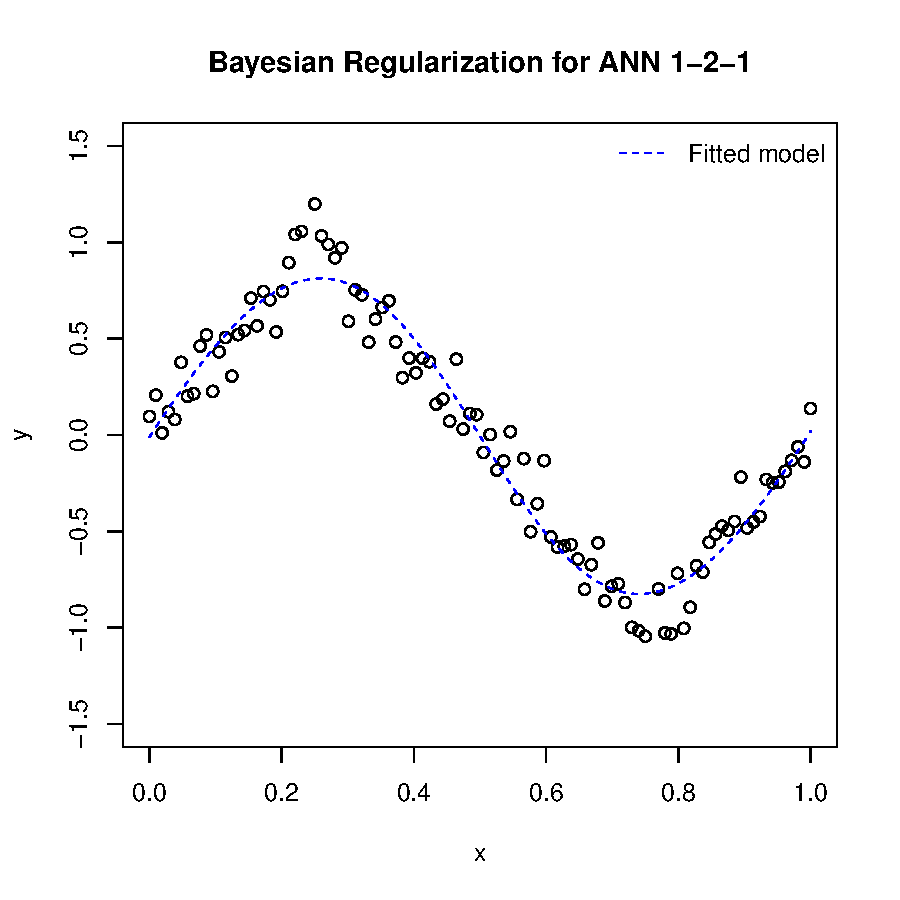
\includegraphics{report-003}
\end{figure}
\section{Tutoriels}
\ntodo[inline]{Encore à voir... on pourrait créer des tutoriels pour peut-être comparer}
\newpage
\begin{appendix}

\section{Code}
\ntodo[inline]{Le code doit aller ici ou faire un autre document. Il peut y avoir des bouts de code dans le texte si cela aide à la compréhension. Le code complet sera fourni à part dans un autre document (pas de limite de pages ici)}
\end{appendix}


\end{document}

